\documentclass[10pt,twocolumn]{scrartcl}

\usepackage{amsmath}

\usepackage{natbib}
\bibliographystyle{plain}

\usepackage{tikz}
\usetikzlibrary{bayesnet}

\renewcommand\phi\varphi

\author{
    Verdegaal Jacob \\
    \texttt{jacob.verdegaal@student.uva.nl}
    \and
    Drumm, Eli\\
    \texttt{etd@dte.li}
    \and
    Noble, Bill\\
    \texttt{winobes@gmail.com}
}

\title{Inducing Semantic Frames on a Very Large Corpus of Syntactic-Ngrams}

\begin{document}

\maketitle

\begin{abstract}
This is the abstract which we will write.
\end{abstract}



\section{Introduction}
Here we provide some background information about what are semantic frames and 
what it menas to induce them and stuff like that.


\section{Related Work}
Here we talk mostly about the O'Connor paper \cite{oconnor2013} and the Rooth 
paper \cite{rooth1999}.


\section{Induction Models}

\subsection{Model 0: Un-structured Tuples}
\begin{tabbing}
    $N$ \hspace{10pt}\= number of data points\\
    $F$              \> number of frames\\
    $\theta$         \> distribution over frames\\
    $\varphi_a$      \> distributions (for each frame) over \\ 
                     \> vocabulary of argument $a$\\
    $w_a$            \> datapoint (verb, subject, object)\\
\end{tabbing}
E-Step:
\begin{equation}
P(f|w_i) = \frac{\prod_a^{\{v,s,o\}}P(w_i^a|\phi_f^a) P(f|\theta)}{\sum_{f'}^F\prod_a^{\{v,s,o\}}P(w_i^a|\phi_{f'}^a)}
\end{equation}
M-Step:
\begin{equation}
P(f|\theta) = \frac{\sum_{i=1}^N \mu_i(f)}{\sum_{f'=1}^F\sum_{i=1}^N\mu_i(f')}
\end{equation}
\begin{equation}
P(w|\phi_f^a) = \frac{\sum_{i=1}^N \mu_i(f) C(w,a)}{\sum_{w'=1}^{V^a}\sum_{i=1}^N \mu_i(f) C(w',a)}
\end{equation}
\begin{tabbing}
    $n$ \hspace{10pt}\= number of data points\\
    $f$              \> number of frames\\
    $v$              \> number of documents (= verb vocabulary)\\
    $\theta$         \> distribution over frames\\
    $\varphi_a$      \> distributions (for each frame) over \\ 
                     \> vocabulary of argument $a$\\
    $w_a$            \> datapoint (verb, subject, object)\\
    $\beta$          \> hyperprior for $\varphi$ (for each argument)\\
    $\alpha$         \> hyperprior for $\theta$ \\
\end{tabbing}

\begin{figure}
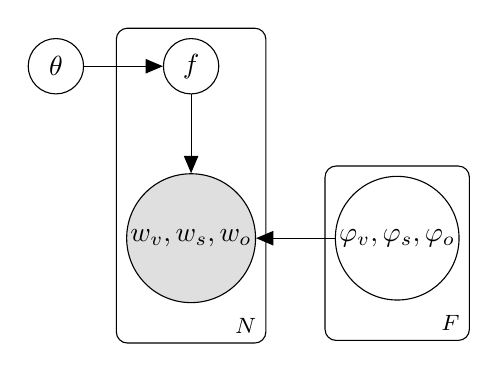
\begin{tikzpicture}
  % Nodes
  \node[obs] (datapoint) {$w_v,w_s,w_o$} ; %
  \node[latent, above=of datapoint] (F) {$f$} ; %
  \node[latent, left=of F] (theta) {$\theta$}; %
  \node[latent, right=of datapoint] (phi) {$\varphi_v,\varphi_s,\varphi_o$}; %
  \edge {theta} {F} ; %
  \edge {F} {datapoint}
  \edge {phi} {datapoint} ; %
  \plate {tuples} {(F) (datapoint) } {$N$}; %
  \plate {} {(phi)} {$F$} ; %
\end{tikzpicture}

\caption{Model 0}
\end{figure}

\subsection{Model 1: Verb Documents}
Gibbs:
\begin{align}
&p(z_{ij} = f| \mathbf{f}_{-ij},\alpha,\beta,\mathbf{w})\\
\propto &\prod_a^{\{v,s,o\}}\frac{\beta^a + \tilde{c}(f,w_{ij})}{V^a + \tilde{c}(f)}
        \cdot \frac{\alpha + \tilde{c}(i,f)}{f\alpha+\tilde{c}(i)}
\end{align}

\begin{tabbing}
    $\tilde{c}(f,w_{ij})$ \hspace{10pt}\= times $w_{ij}$ is assigned to frame $f$\\
    $\tilde{c}(f)$                     \> total data points assigend to $f$\\
    $\tilde{c}(i,f)$                   \> VSOs in document $i$ assigned to $f$\\
    $\tilde{c}(i)$                     \> VSOs in document $i$\\ 
\end{tabbing}

\begin{figure}
    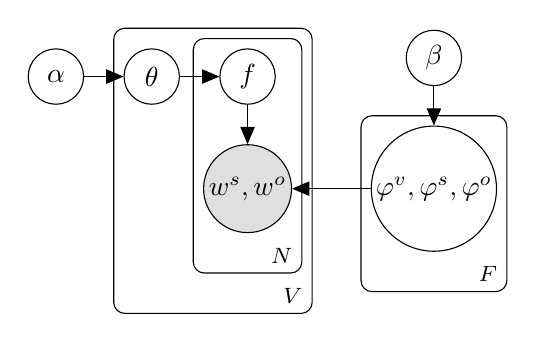
\begin{tikzpicture}[]
    \node[obs]                   (w)     {$w^s,w^o$}; %
    \node[latent, above=0.5cm of w]     (f)     {$f$};
    \node[latent, left=0.5cm of f]     (theta) {$\theta$};
    \node[latent, left=0.5cm of theta] (alpha) {$\alpha$};
    \node[latent, right=of w]    (phi)   {$\varphi^v,\varphi^s,\varphi^o$};
    \node[latent, above=0.5cm of phi] (beta) {$\beta$};
    \edge {alpha} {theta};
    \edge {theta} {f};
    \edge {f} {w};
    \edge {phi} {w};
    \edge {beta} {phi};
    \plate {frames} {(phi)} {$F$};
    \plate {datapoints} {(f) (w)} {$N$};
    \plate {verbs} {(f) (w) (datapoints) (theta)} {$V$};
\end{tikzpicture}

    \caption{Model 1}
\end{figure}


\section{Data}

\subsection{Google Syntactic-ngrams}
Here we talk a bit about the syntactic n-grams and all that \cite{ngrams2013}.
\begin{itemize}
    \item A syntactic-ngram is a $k$-word rooted subtree for some sentence. 
    \item Google ngrams come from a corpus of 3.5 million English books.
    \item We trimmed the ``verb args'' dataset to consider only subject-verb-object triples (VSO's).
    \item The dataset contains 1,629,120 unique VSO's with a total of 96,245,401 by count.
    \item In our final results we may only use the most common \%20 of these...
\end{itemize}

\subsection{Pruning}


\section{Experiments}


\section{Results}
\subsection{Frame Coherency}
rame coherency: for a datapoint $(v,s,o)$ and a tuple $(v^r,s,o)$ where $v^r$ is a random choses verb: $P(v\mid s,o) \geq P(v^r\mid s,o)$  
\subsection{Frame Correctness}
Frame correctness: for the top 25 most probable verbs per frame $TV$ and framenet classes of verbs $FN$: \[\frac{2|TV\cap FN|}{|TV|+|FN|}\]
\subsection{Model 0}
\subsection{Model 1}


\section{Discussion}


\section{Future Work}


\section{Conclusion}


\bibliography{refs.bib}
\end{document}
